\subsection{Track reconstruction in pp collisions}

Standard track reconstruction in CMS occurs in the following steps, summarized here and described in detail in Ref.~~\cite{Chatrchyan:2014fea}: 
\begin{itemize}
\item \textbf{Hit reconstruction} --  In the pixel tracker, zero-supression is performed by setting an adjustable threshold, equivalent charge to 3200 for each pixel. Pixel its are reconstructed as clusters of adjacent pixels, requiring a minimum charge equivalent of 4000 electrons (compared to at least 21,000 electrons deposited by a typical ionizing particle).  In the strip detector, zero-suppression is performed by subtracting the baseline pedestal and noise from the signal, and clusters are seeded with channels which contain charge at least three times that of the pedestal.  Adjacent strips are added to the cluster if their charge is more than twice that of the pedestal, and the cluster is kept if its total charge is at least five times larger than the combined strip noise.  Cluster position in the strip detector is determined from the charge-weighted average of strip positions, corrected for Lorentz drift.  The average efficiency for hit reconstruction in both the pixel and strip detectors (excluding 2.4\% of pixel modules and 2.3\% of strip modules known to be defective) is $> 99$ \%.

\item \textbf{Track seed generation}  -- Track reconstruction begins by first running a fast track and vertex reconstruction using the pixel tracker only to reconstruct the beamspot position and the location of primary vertices in the event.  After this, track reconstruction is carried out in six iterations, each of which begins with ``seeds'' that define the trajectories and uncertainties of potential tracks.  The first set of seeds are pixel triplets, produced from corresponding sets of three pixel hits (on a helical track trajectory) with weak constraints on ompatibility with the beam spot to require that the tracks correspond to promptly produced particles.  In later iterations, additional information from vertex reconstruction and the silicon strip detector is incorporated in seed generation.

\item \textbf{Track finding} -- The seeds generated in the step above are used as starting points for track-finding based on the Kalman filter method, implemented in four steps for each tracker layer.  First, track parameters at the starting level are extrapolated, assuming a perfectly helical track trajectory (neglecting multiple scatterings, energy loss, and non-uniformity in the magnetic field), to determine the locations of interception in other pixel layers.  The second step is a search for tracker modules consistent with the interception locations determined in the previous step.  In the third step, hits from mutually exclusive module groups (i.e. groups of modules for which it is not possible that one track could pass through more than one of the grouped modules) are used to update and refine hit locations (including the possibility of adding ``ghost'' hits where a particle failed to produce a hit due to module inefficiency) and to calculate the Lorentz drift in the silicon bulk.  Finally, in the fourth and last step, new track candidates are formed by adding one compatible hit from each of the module groupings, and trajectories are updated combining this added hit with the original track path extrapolation.  All track candidates at a given level are then extrapolated to the next compatible layer and the procedure repeated through five iterations.

\item \textbf{Track fitting} -- Finally, the track trajectory is refitted to reduce possible biases (due, for example, to the beam spot constraint introduced in initial seed finding), and to remove outlying hits falsely associated to a track.  

\end{itemize}

\noindent After tracks are reconstructed according to this procedure, the track sample both includes a contribution from ``fake'' tracks (that do not correspond to the trajectory of an ionizing particle), which is reduced by requiring certain selection criteria as discussed in Sec.~\ref{sec:high_purity}.  The collection also suffers from detector and reconstruction inefficiencies, which are corrected in this analysis according to the procedure described in Sec.~\ref{sec:track_eff}.

\subsection{Track reconstruction in PbPb collisions}

In PbPb collision data, dedicated track reconstruction is necessary due to the dramatically greater multiplicity in PbPb compared to pp collisions.  This heavy ion tracking occurs in the following steps, and is detailed in Refs.~\cite{AN_2014_024} and~\cite{AN-15-187}: 
\begin{itemize}

\item \textbf{Hit reconstruction} -- Tracker hits are reconstructed following the same basic procedure applied in pp collisions.

\item \textbf{Track seed generation} -- First, primary vertex positions are reconstructed using only a collection of pixel hits, extrapolated to the region near the beam spot.  In PbPb data pileup is negligible, so there is generally only one primary vertex reconstructed in each event.  Initial track seeds are then constructed from pixel triplets only.  To reduce combinatorial backgrounds, seeds are restricted to those pointing to a region within 2 mm of the primary vertex, and further selections are applied on track $p_{\rm T}$, goodness-of-fit ($\chi^{2}$), and compatibility between the seed trajectory and the primary vertex.  

\item \textbf{Track finding} -- Track trajectories are propagated through the tracker following a procedure similar to that outlined above for pp data.  The track seeding and finding procedure is repeated through three iterations.  In the second and third iterations, hits belonging unambigulously to a previously identified tracks are first removed, and then reconstruction is repeated using pixel triplet and pixel pair seeds (in the 2nd and 3rd iterations, respectively).  Tracks identified in these later iterations are merged into first-iteration tracks, with duplicates removed based on hit matching.

\end{itemize}

\subsection{High purity tracks}
\label{sec:high_purity}

The track reconstruction procedures described above for pp and PbPb collision data give track collections with significant ``fake rates,'' or fraction of reconstructed tracks that cannot be associated with a particle.  This fake rate is reduced with a series of quality selections, defined in three levels:  ``loose'' criteria define the minimum to keep tracks in track collections, ``tight'' criteria are somewhat more stringent (sacrificing some lost efficiency for a lower fake rate), and finally ``high purity'' criteria are most strict and are those applied for most CMS analyses, including those reported here.  Track quality in each case is set with flags for each track, and criteria in each case are applied separately at each iterative tracking step.  The precise criteria for high purity tracks at each iterative pass are defined in Refs.~\cite{Chatrchyan:2014fea, AN_2014_024, AN-15-187}, and include the following types of selections, imposed as a function of $p_{\rm T}$ and $\eta$: 

\begin{itemize}
\item Requirements on the number of hits on the track trajectory ($N_{\rm hit}$)
\item Requirements on the minimum layers in which the track has an associated hit ($N_{\rm layers}$, and on the maximum intercepted layers in which the track has no assigned hits
\item A minimum imposed on the goodness-of-fit of the track ($\chi^{2}/\rm{Ndof}/N_{\rm layers}$ or $\chi^{2}/N_{\rm hit}$)
\item A maximum on relative track-$p_{\rm T}$ uncertainty
\item Maxima on longitudinal and transverse impact parameters ($\rm d_{z}$ and $\rm d_{xy}$) with respect to the primary vertex position and beam spot
\end{itemize}

\noindent In pp data, criteria are optimized by the quality metric $Q(\rho) = s/ \sqrt{s+\rho b}$, where s = selected (``real'') tracks, b = selected fake tracks, and parameter $\rho \approx  10$ weights the metric toward minimizing the fake rate.  In PbPb data from Run 2, optimization is performed via the output of a multivariate analysis tool (MVA), as detailed in Ref.~\cite{AN-15-187}.

\subsection{Tracking efficiency and fake rate evaluation and correction}
\label{sec:track_eff}

Tracking efficiency for charged particles in pp collisions ranges from approximately 80\% at $p_{\rm T}\approx$0.5~GeV to 90\% or better at $p_{\rm T}\approx$10~GeV and higher.  Track reconstruction is more difficult in the heavy-ion environment due to the high track multiplicity, and tracking efficiency for PbPb collisions ranges from approximately 30\% at 0.5~GeV to about 70\% at 10~GeV.  Tracking efficiencies are evaluated using {\sc pythia} and {\sc pythia+hydjet} Monte Carlo simulation, by comparing track distributions as generated to those after MC samples are passed through {\sc Geant} detector simulation and reconstructed with the algorithms used to reconstruct data.  Corrections are derived as a function of centrality, $p_{\rm T}$, $\eta$, $\phi$, and local charged particle density.   Tracking efficiency closure and systematic uncertainty is evaluated in {\rm pythia} and {\rm pythia+hydjet}, comparing generated track $p_{\rm T}$, $\eta$, and $\phi$ distributions to reconstructed distributions before and after correction.  For illustration, examples of these closure checks for 5.02 TeV {\sc pythia} simulation are shown in Fig.~\ref{fig:trk_eff_pythia}.  Additional 5\% residual systematic uncertainty is conservatively assigned for possible differences between MC and data that might affect tracking performance.  


 \begin{figure}[h!]
    \begin{center}
       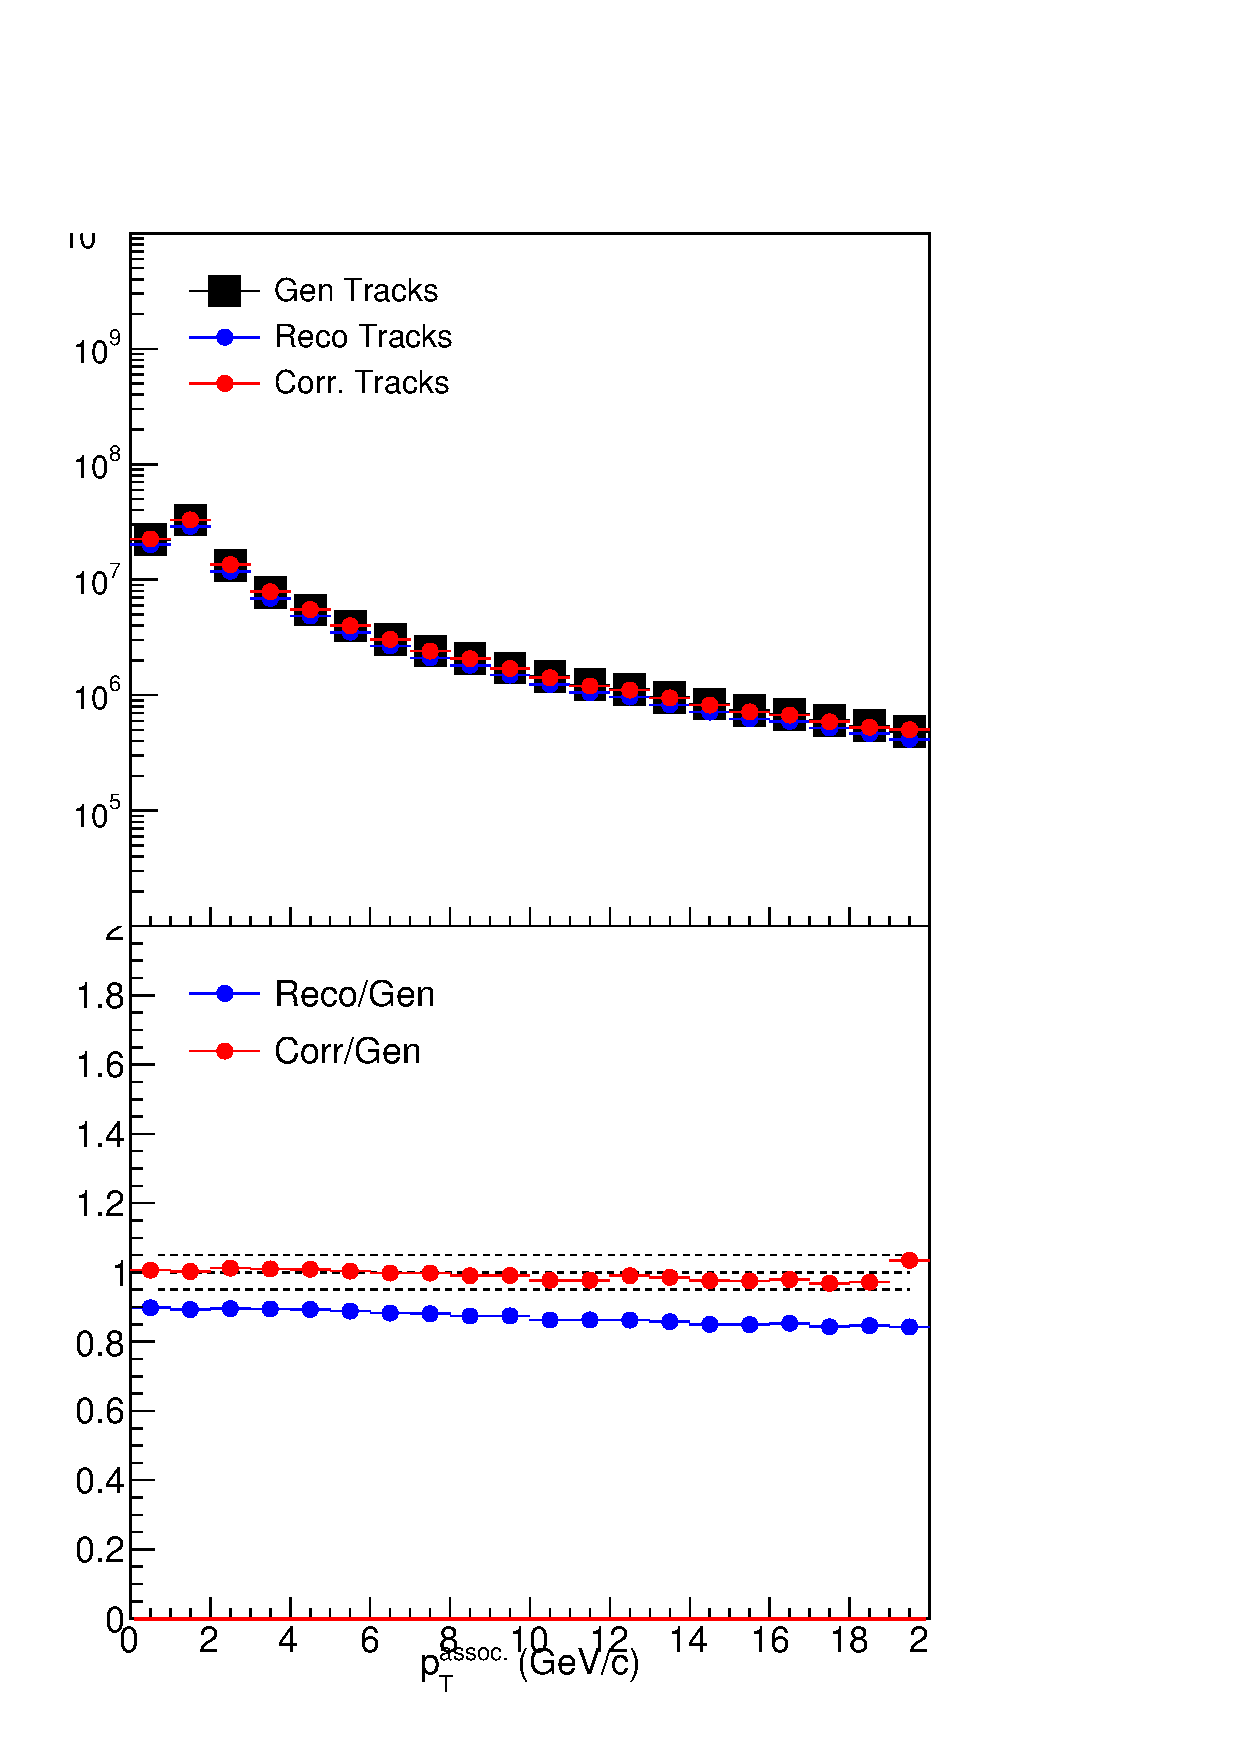
\includegraphics[width=0.299\textwidth]{figures/Detector/TrackingEfficiencyPtPythia.pdf}
             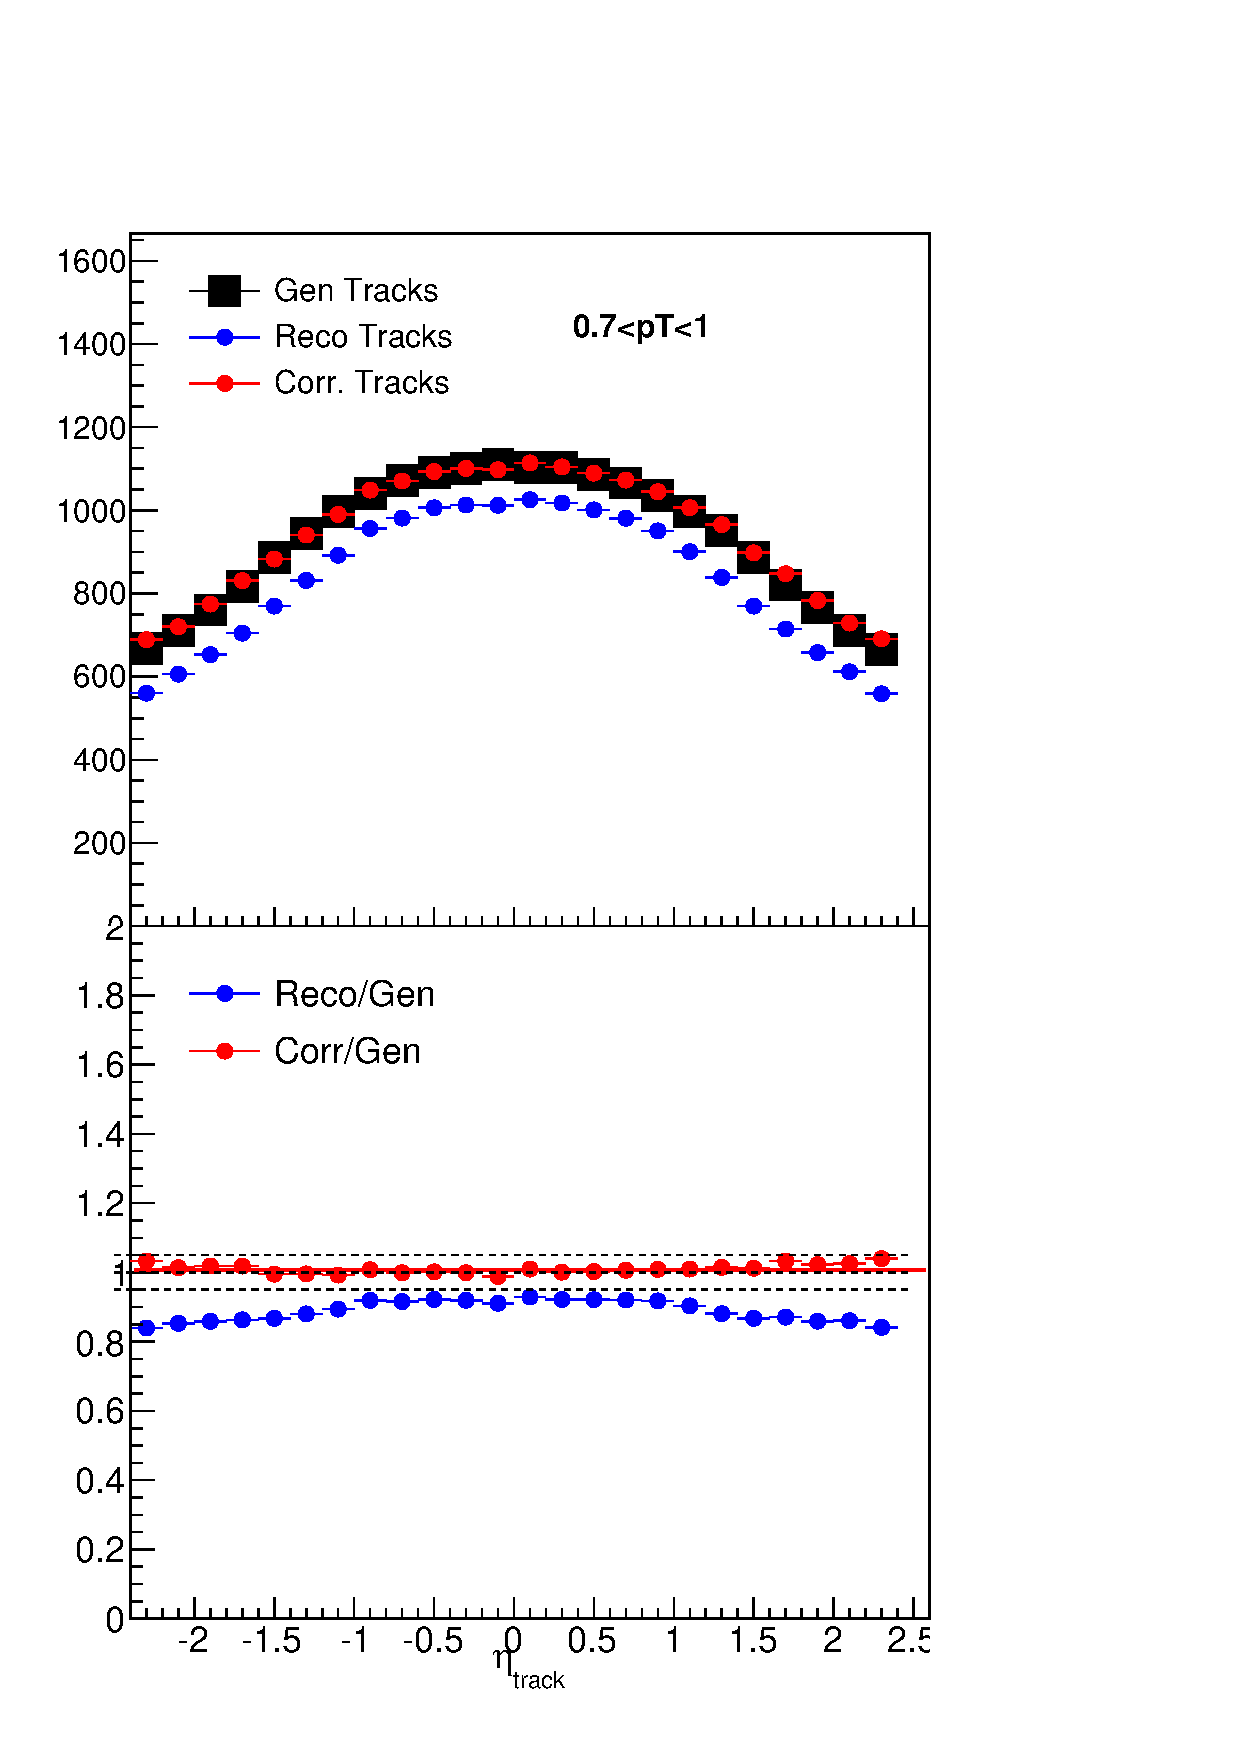
\includegraphics[width=0.299\textwidth]{figures/Detector/TrackingEfficiencyEtaPythia_TrkPt0p7TrkPt1.pdf}	
                    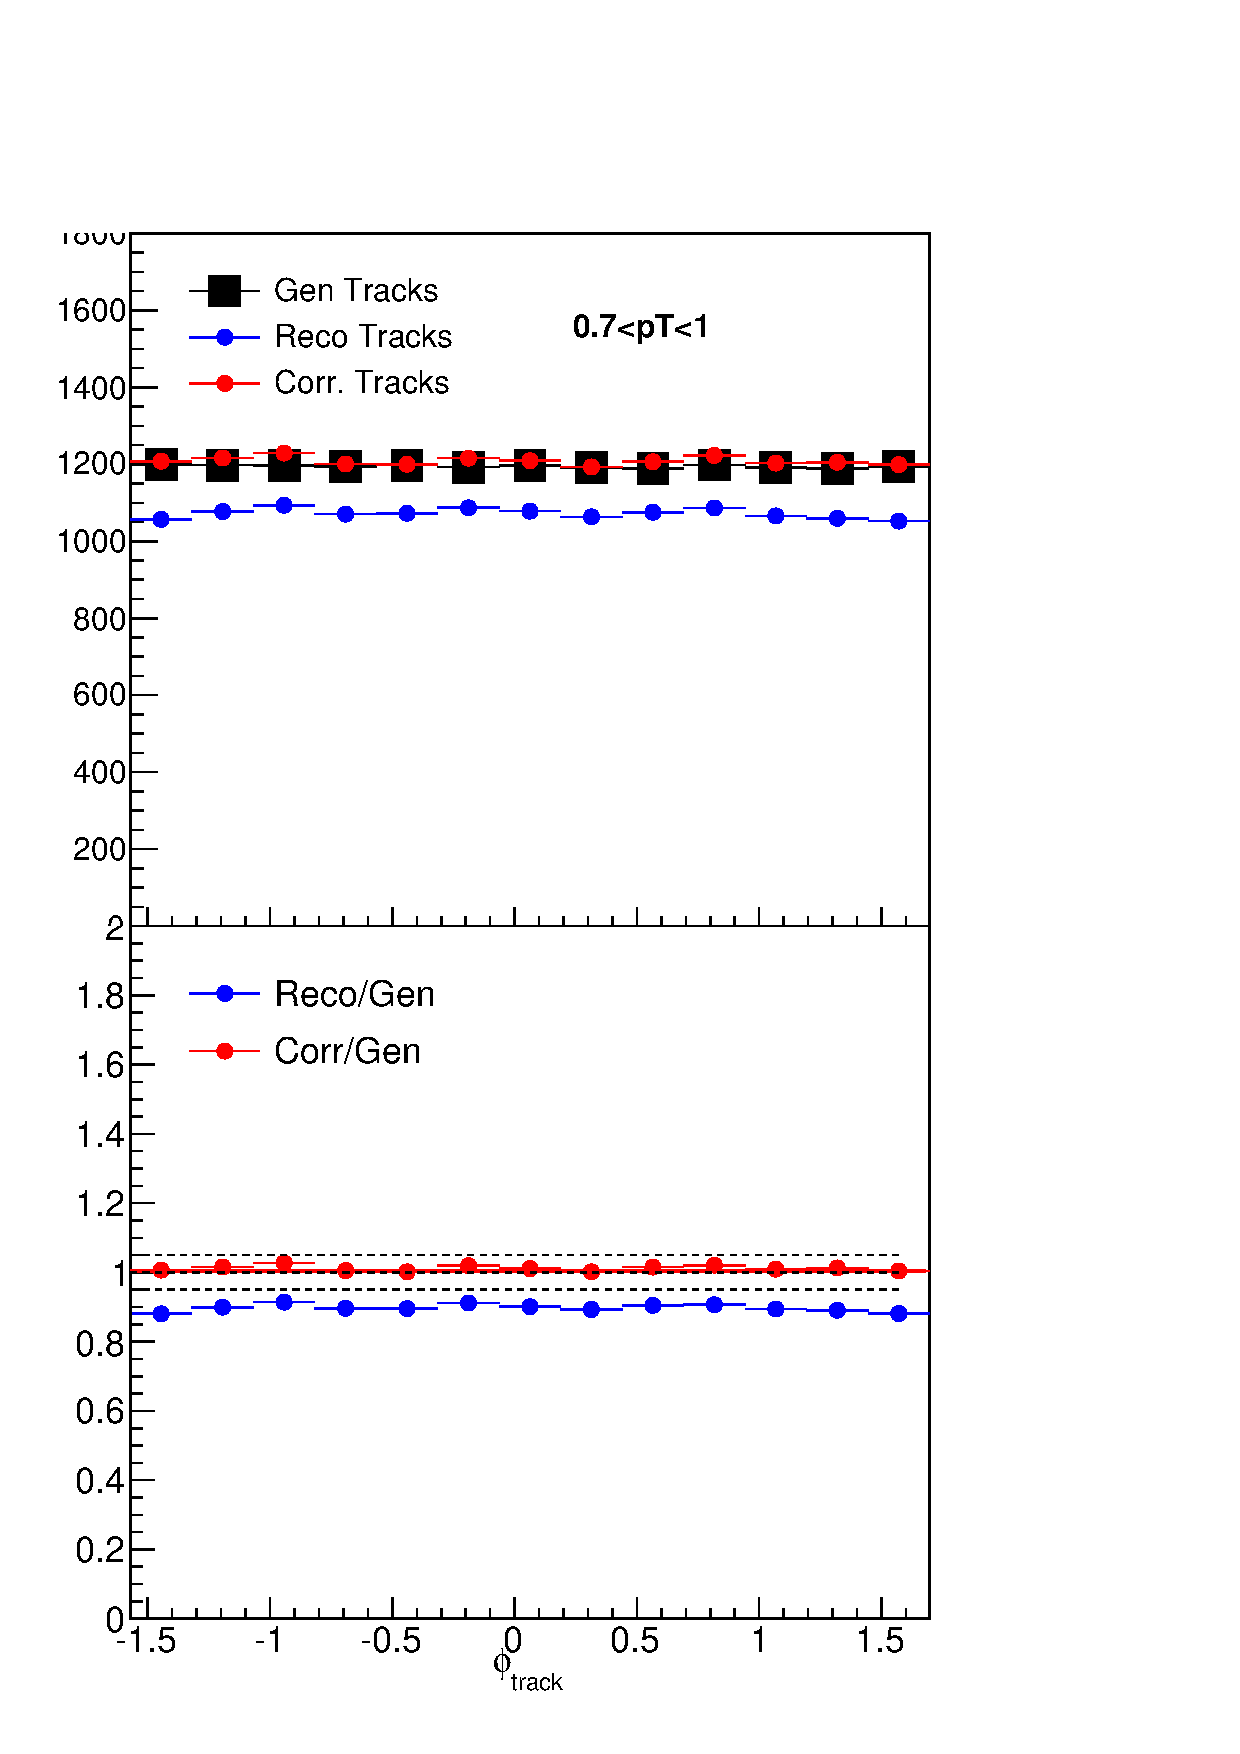
\includegraphics[width=0.299\textwidth]{figures/Detector/TrackingEfficiencyPhiPythia_TrkPt0p7TrkPt1.pdf}	
         \caption[Tracking efficiency correction example]{Tracking efficiency correction closure for {\sc pythia} simulation at 5.02 TeV, comparing tracking generated tracks to uncorrected and corrected reconstructed tracks, as a function of track $p_{\rm T}$ and of pseudorapidity, and azimuth for the lowest $p_{\rm T}^{\rm trk}$ bin.}
       \label{fig:trk_eff_pythia}
    \end{center}
 \end{figure}
 
 



